\chapter{Wstęp}

\section{Cel pracy}
Celem projektu inżynierskiego jest opracowanie programu opartego na uczeniu maszynowym, zdolnego do samodzielnego rozwiązywania problemów występujących w grze \textit{Super Mario Bros} na platformie Nintendo Entertainment System (NES).
Projekt obejmuje badanie zastosowania algorytmów uczenia ze wzmocnieniem oraz analizę efektywności różnych podejść w symulowanym środowisku gry.

\section{Opis gry \textit{Super Mario Bros}}

\textit{Super Mario Bros} to klasyczna gra platformowa wydana przez Nintendo w 1985 roku na konsolę NES.
Celem gry jest przejście bohaterem, Mario, z lewej strony ekranu na prawą, aż do końca poziomu, gdzie zwykle znajduje się flaga oznaczająca jego ukończenie.
Gracz musi pokonać serię poziomów.

Podczas gry Mario napotyka różnorodne przeszkody, wrogów oraz pułapki.
Do głównych zagrożeń należą przeciwnicy, tacy jak Goomba i Koopa Troopa, przepaście oraz spadające platformy.
Aby unikać zagrożeń lub je eliminować, Mario może skakać na wrogów lub korzystać z przedmiotów zwiększających jego zdolności, takich jak grzyby, które powiększają postać, czy kwiaty ognia umożliwiające atakowanie przeciwników z dystansu.

Kluczową mechaniką gry jest precyzyjne poruszanie się i planowanie kolejnych ruchów, ponieważ niewłaściwe decyzje często prowadzą do przegranej.

\begin{figure}[h!]
    \centering
    \includegraphics[width=0.8\textwidth]{img/screenshot_mario.png}
    \caption{Przykładowy ekran z gry \textit{Super Mario Bros.}}
    \label{fig:screenshot_mario}
\end{figure}

\subsection{Kontroler NES}

Do gry wykorzystywany jest prosty kontroler NES. Posiada on cztery przyciski kierunkowe (góra, dół, lewo, prawo) oraz dwa przyciski akcji oznaczone jako \textit{A} i \textit{B}. Przyciski te pozwalają na wykonywanie takich czynności jak skakanie, bieganie i atakowanie przeciwników.


\begin{figure}[h!]
    \centering
    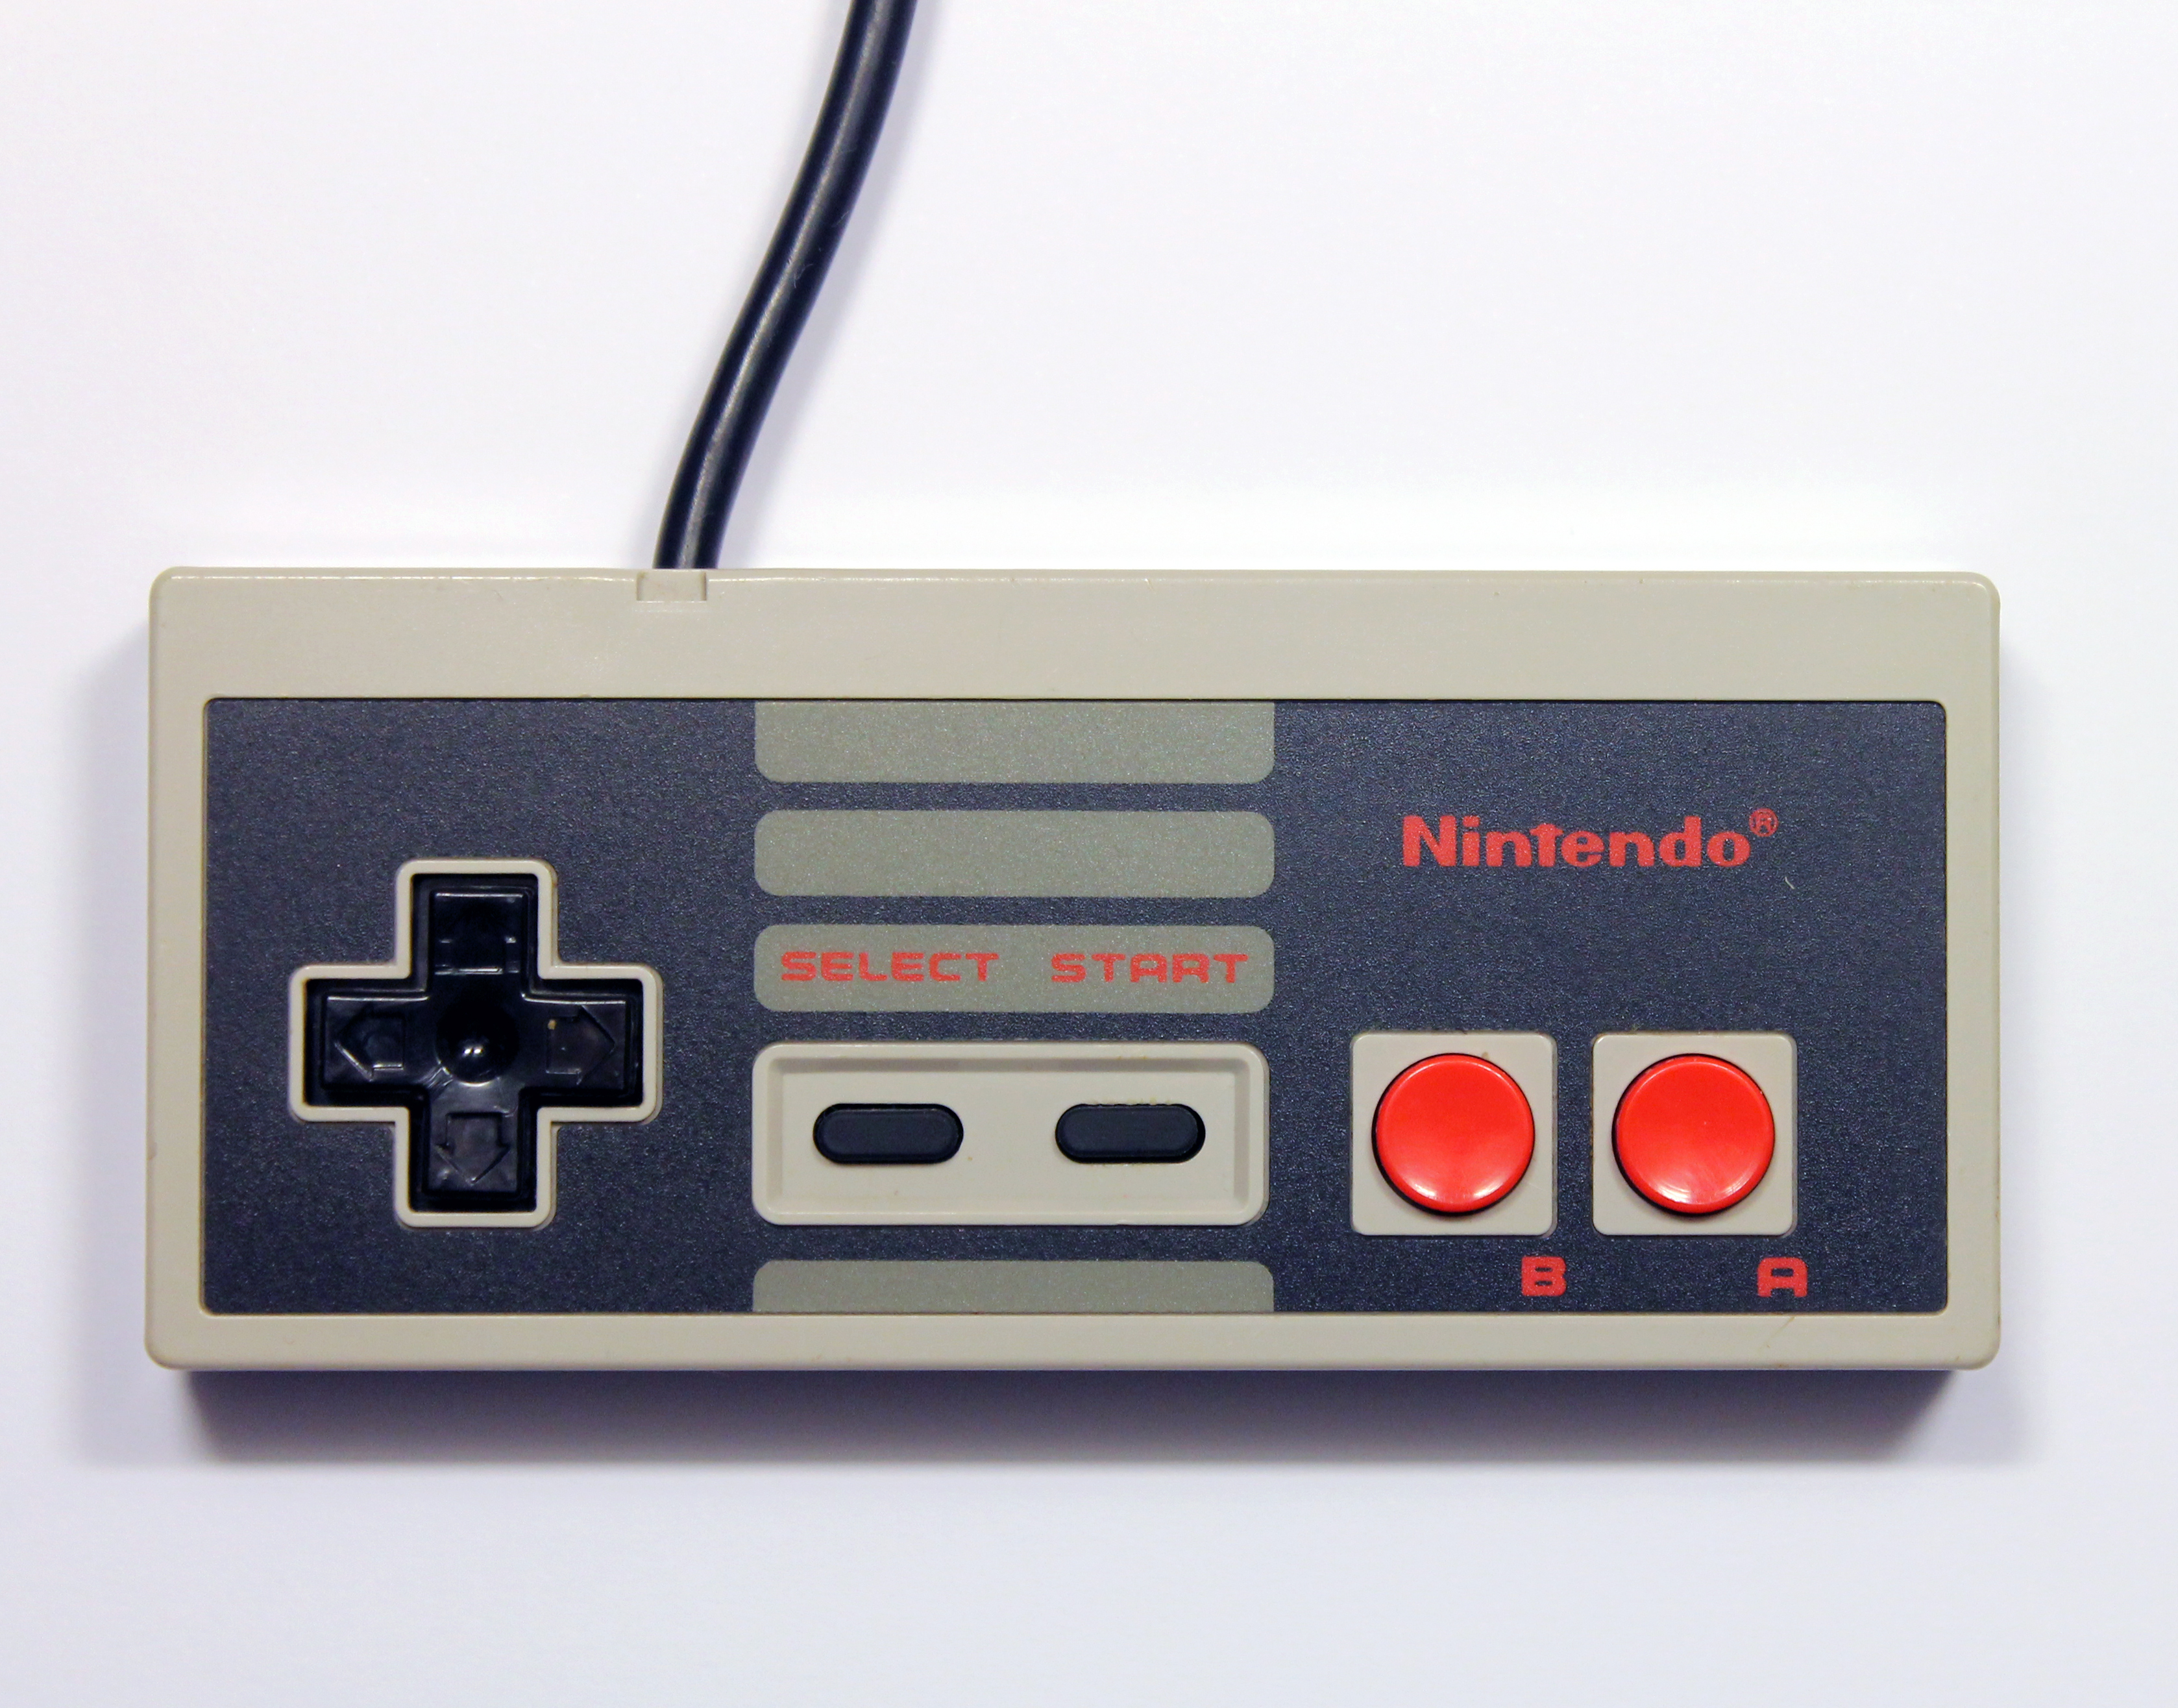
\includegraphics[width=0.5\textwidth]{img/nes_controller.JPG}
    \caption{Kontroler NES używany w grze Super Mario Bros.\\Denis Apel / \url{flyingpixel.de} / Wikipedia}
    \label{fig:nes_controller}
\end{figure}

\section{Zakres pracy}
Celem niniejszej pracy jest stworzenie programu, który nauczy model sztucznej inteligencji skutecznego przechodzenia wybranego poziomu gry Super Mario Bros. Projekt obejmuje:
\begin{itemize}
    \item opracowanie środowiska umożliwiającego interakcję z emulatorem NES,
    \item implementację algorytmu Double Q-Learning,
    \item przeprowadzenie eksperymentów oceniających efektywność modelu.
\end{itemize}
Zakres pracy ogranicza się do jednego wybranego poziomu gry, z pominięciem aspektów dźwięku oraz rozgrywki wielopoziomowej.
